% !TeX program = pdflatex
\documentclass[12pt,a4paper]{article}

% =====================================
%         USTAWIENIA I PAKIETY
% =====================================
\usepackage[utf8]{inputenc}
\usepackage[T1]{fontenc}
\usepackage[polish]{babel}
\usepackage{graphicx}
\usepackage{amsmath, amssymb}
\usepackage{float}
\usepackage{geometry}
\usepackage{booktabs}
\usepackage{caption}
\usepackage{subcaption}
\usepackage{pgfplots}
\usepackage{hyperref}
\usepackage{icomma} % Poprawne przecinki w trybie matematycznym

\geometry{margin=2.5cm}
\setlength{\parindent}{1.2cm}
\setlength{\parskip}{0.5em}
\linespread{1.2}

\pgfplotsset{compat=1.18}

% Ustawienia dla hyperref (opcjonalne, ale poprawia wygląd PDF)
\hypersetup{
	colorlinks=true,
	linkcolor=black,
	filecolor=black,      
	urlcolor=blue,
	pdftitle={Sprawozdanie SA - Cw 1},
	pdfpagemode=FullScreen,
}

% =====================================
%          DOKUMENT
% =====================================
\begin{document}
	
	% =====================================
	%          STRONA TYTUŁOWA
	% =====================================
	\begin{titlepage}
		\centering
		\Huge \textbf{Sprawozdanie z ćwiczeń laboratoryjnych}\\[0.5cm]
		\Large z przedmiotu: \textit{Sterowanie Analogowe}\\[2cm]
		
		\begin{tabular}{|p{6cm}|p{10cm}|}
			\hline
			\textbf{Numer ćwiczenia:} & 1 \\
			\hline
			\textbf{Tytuł ćwiczenia:} & Identyfikacja obiektów dynamicznych \\
			\hline
			\textbf{Imię, nazwisko i numer albumu:} & 
			\begin{tabular}[t]{@{}l@{}}
				Mateusz Kuczerowski 197900\\
				Kewin Kisiel 197866\\
			\end{tabular} \\
			\hline
			\textbf{Data pomiarów:} & 9.10.2025 \\
			\hline
			\textbf{Data oddania:} & 15.10.2025 \\
			\hline
			\textbf{Ocena:} & \\
			\hline
		\end{tabular}\\[2cm]
		
		\vfill
		\textbf{Prowadzący:} dr inż. Piotr Fiertek\\[0.2cm]
		\textbf{Grupa laboratoryjna:} 1A\\[1cm]
	\end{titlepage}
	
	% =====================================
	%          CEL ĆWICZENIA
	% =====================================
	\section{Cel ćwiczenia}
	Celem ćwiczenia było zapoznanie się z czasowymi i częstotliwościowymi metodami identyfikacji obiektów dynamicznych oraz praktyczne wyznaczenie modeli matematycznych opisujących ich zachowanie. W ramach zajęć analizowano odpowiedzi różnych typów układów dynamicznych na wymuszenia skokowe i sygnały harmoniczne, co pozwoliło na określenie ich podstawowych parametrów, takich jak wzmocnienie, stała czasowa, opóźnienie transportowe, współczynnik tłumienia czy pulsacja naturalna.
	
	% =====================================
	%          PRZEBIEG ĆWICZENIA
	% =====================================
	\section{Przebieg ćwiczenia}
	Podczas ćwiczenia przeprowadzono identyfikację kilku obiektów dynamicznych o znanych transmitancjach operatorowych: układu inercyjnego pierwszego rzędu, układu inercyjnego pierwszego rzędu z opóźnieniem transportowym, układu całkującego, układu drugiego rzędu oraz układu nieminimalnofazowego. Dla każdego z nich wykonano pomiary odpowiedzi czasowych oraz charakterystyk częstotliwościowych (amplitudowych i fazowych). W trakcie zajęć wykorzystano stanowisko pomiarowe zbudowane z zestawu analogowych modeli procesów przemysłowych (ZAMPP), generatora funkcji, częstościomierza oraz oscyloskopu dwukanałowego. Zarejestrowane dane zostały następnie przetworzone i poddane analizie w środowisku MATLAB, gdzie z użyciem odpowiednich skryptów dokonano numerycznej identyfikacji parametrów poszczególnych modeli.
	
	% =====================================
	%          ANALIZA I WYNIKI
	% =====================================
	\newpage
	\section{Pomiary i analiza wyników}
	Poniżej przedstawiono zdjęcia z przeprowadzonych pomiarów w trakcie laboratorium.
	
	\begin{figure}[H]
		\centering
		\begin{subfigure}[b]{0.48\textwidth}
			\centering
			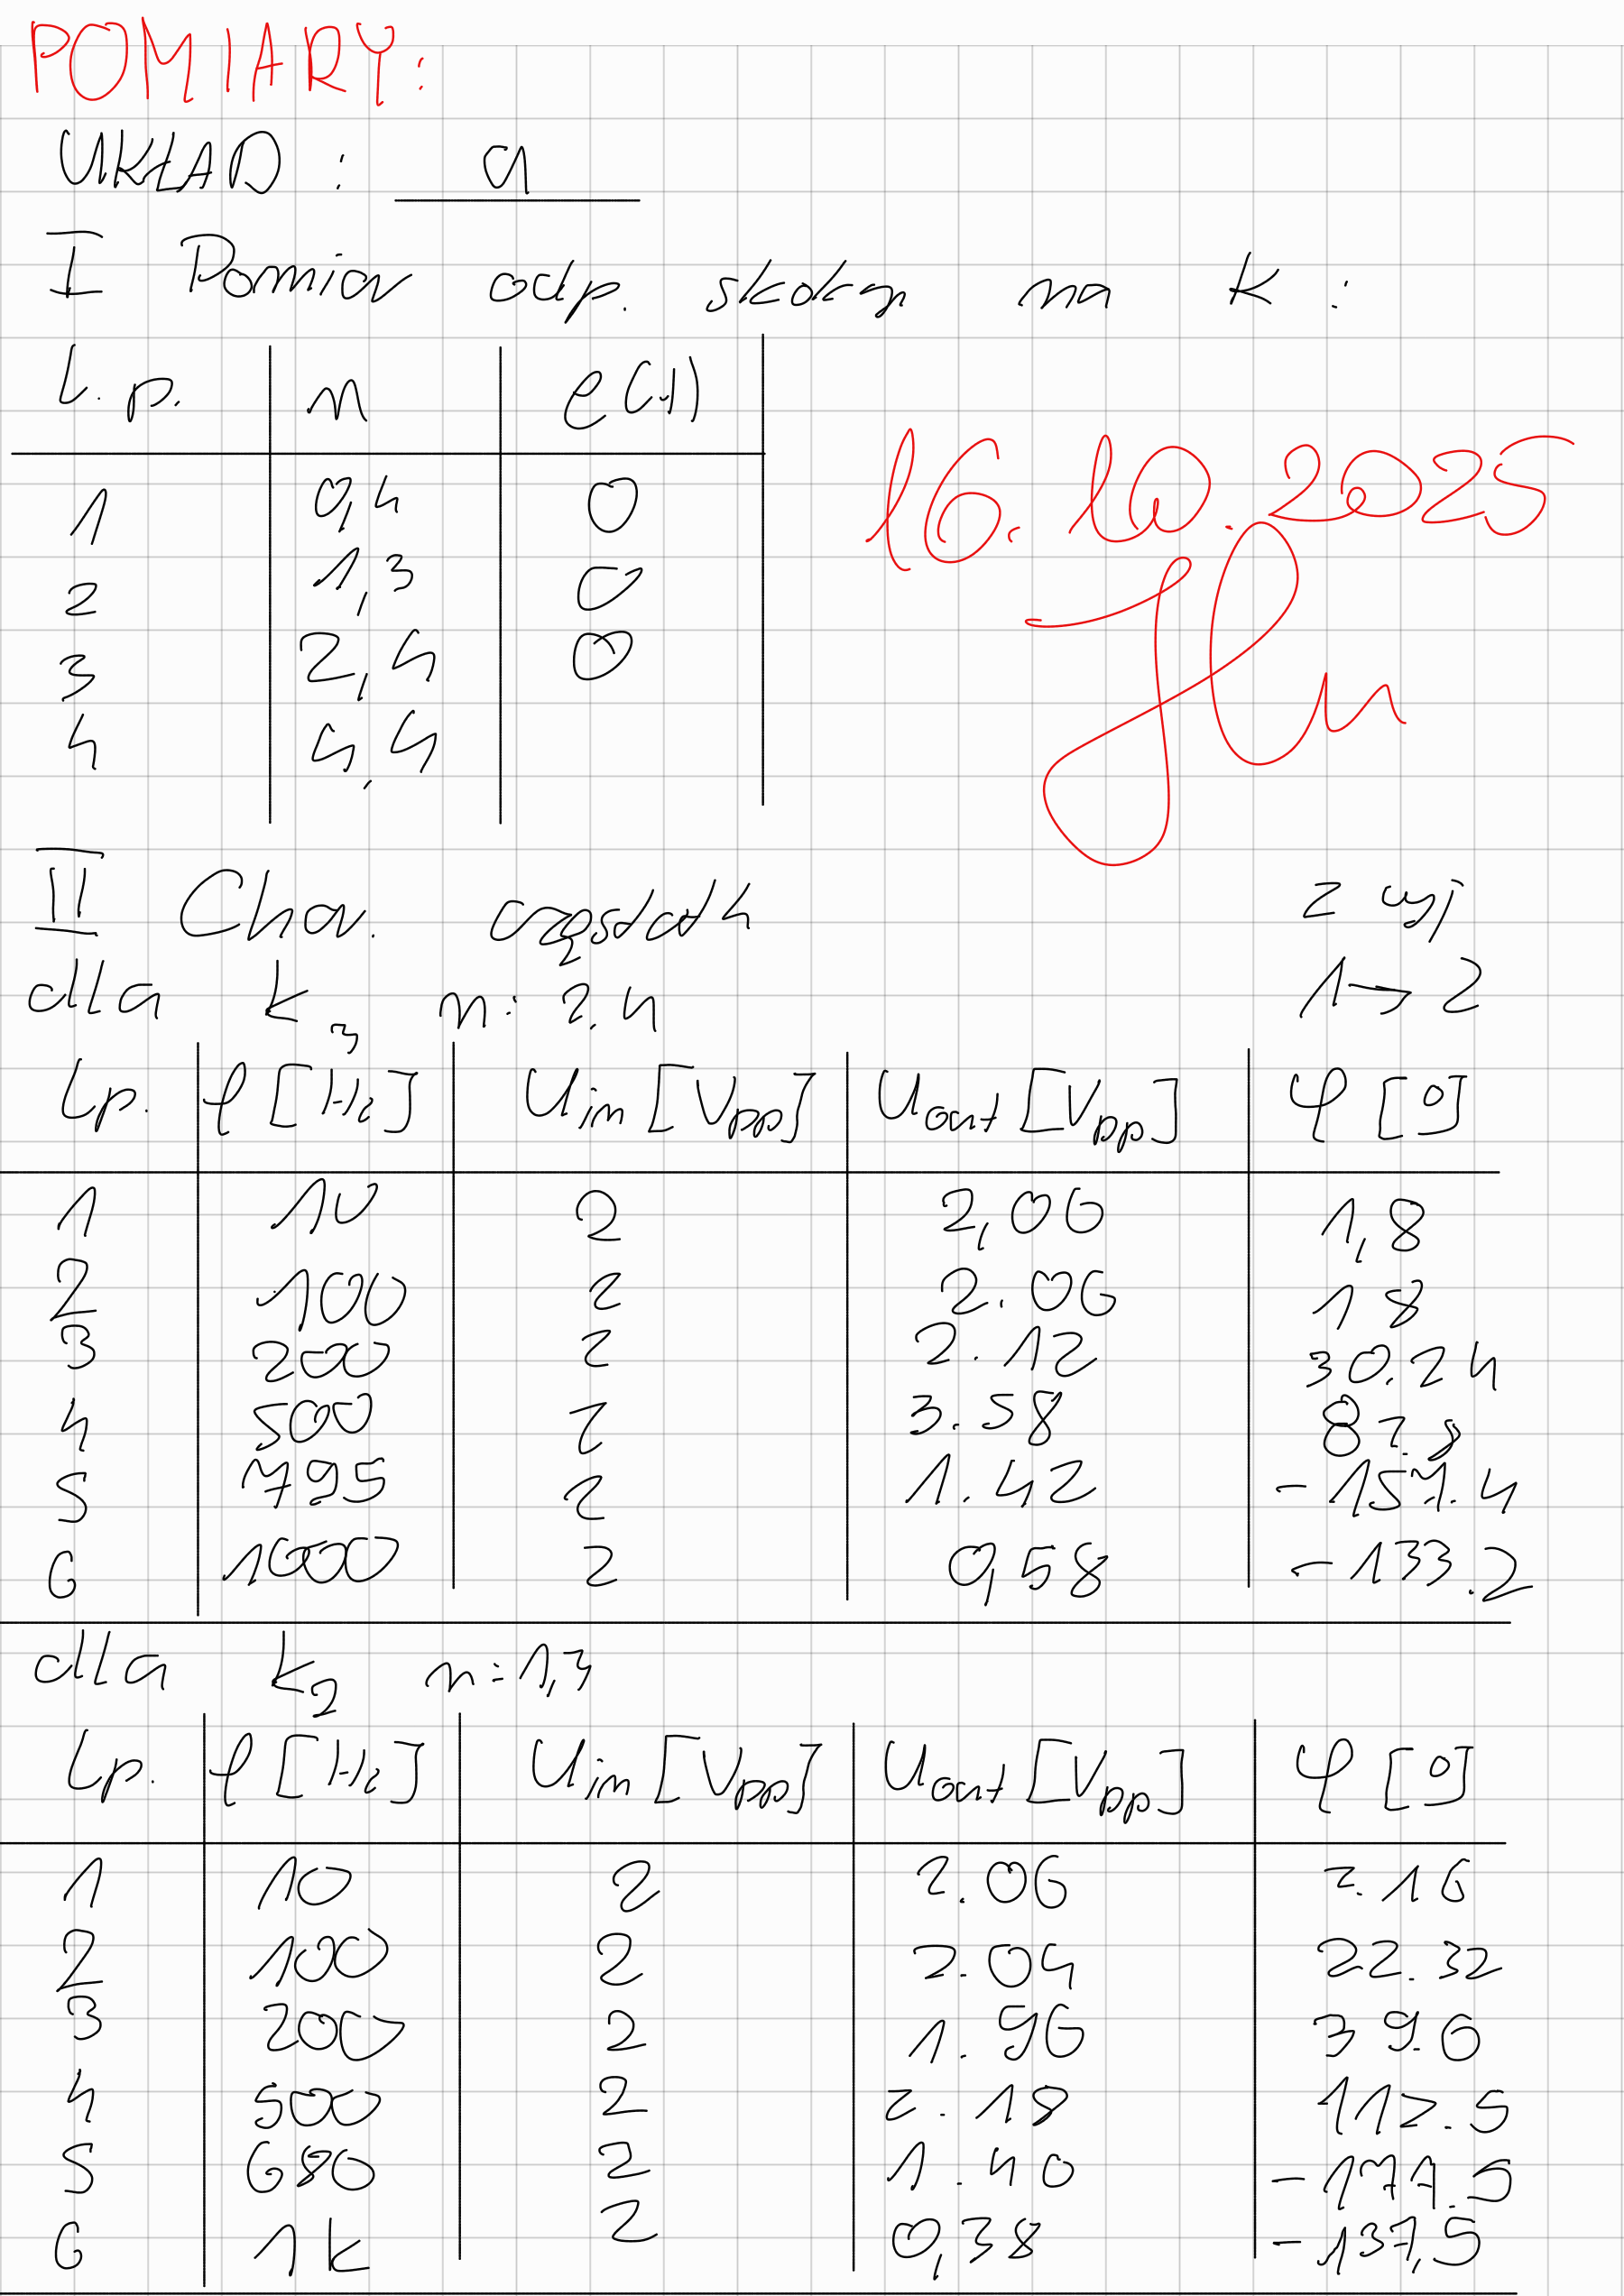
\includegraphics[width=\textwidth]{zdjecia/1.png}
			\caption{Zdjęcie pomiarów 1.}
			\label{fig:pomiar1}
		\end{subfigure}
		\hfill
		\begin{subfigure}[b]{0.48\textwidth}
			\centering
			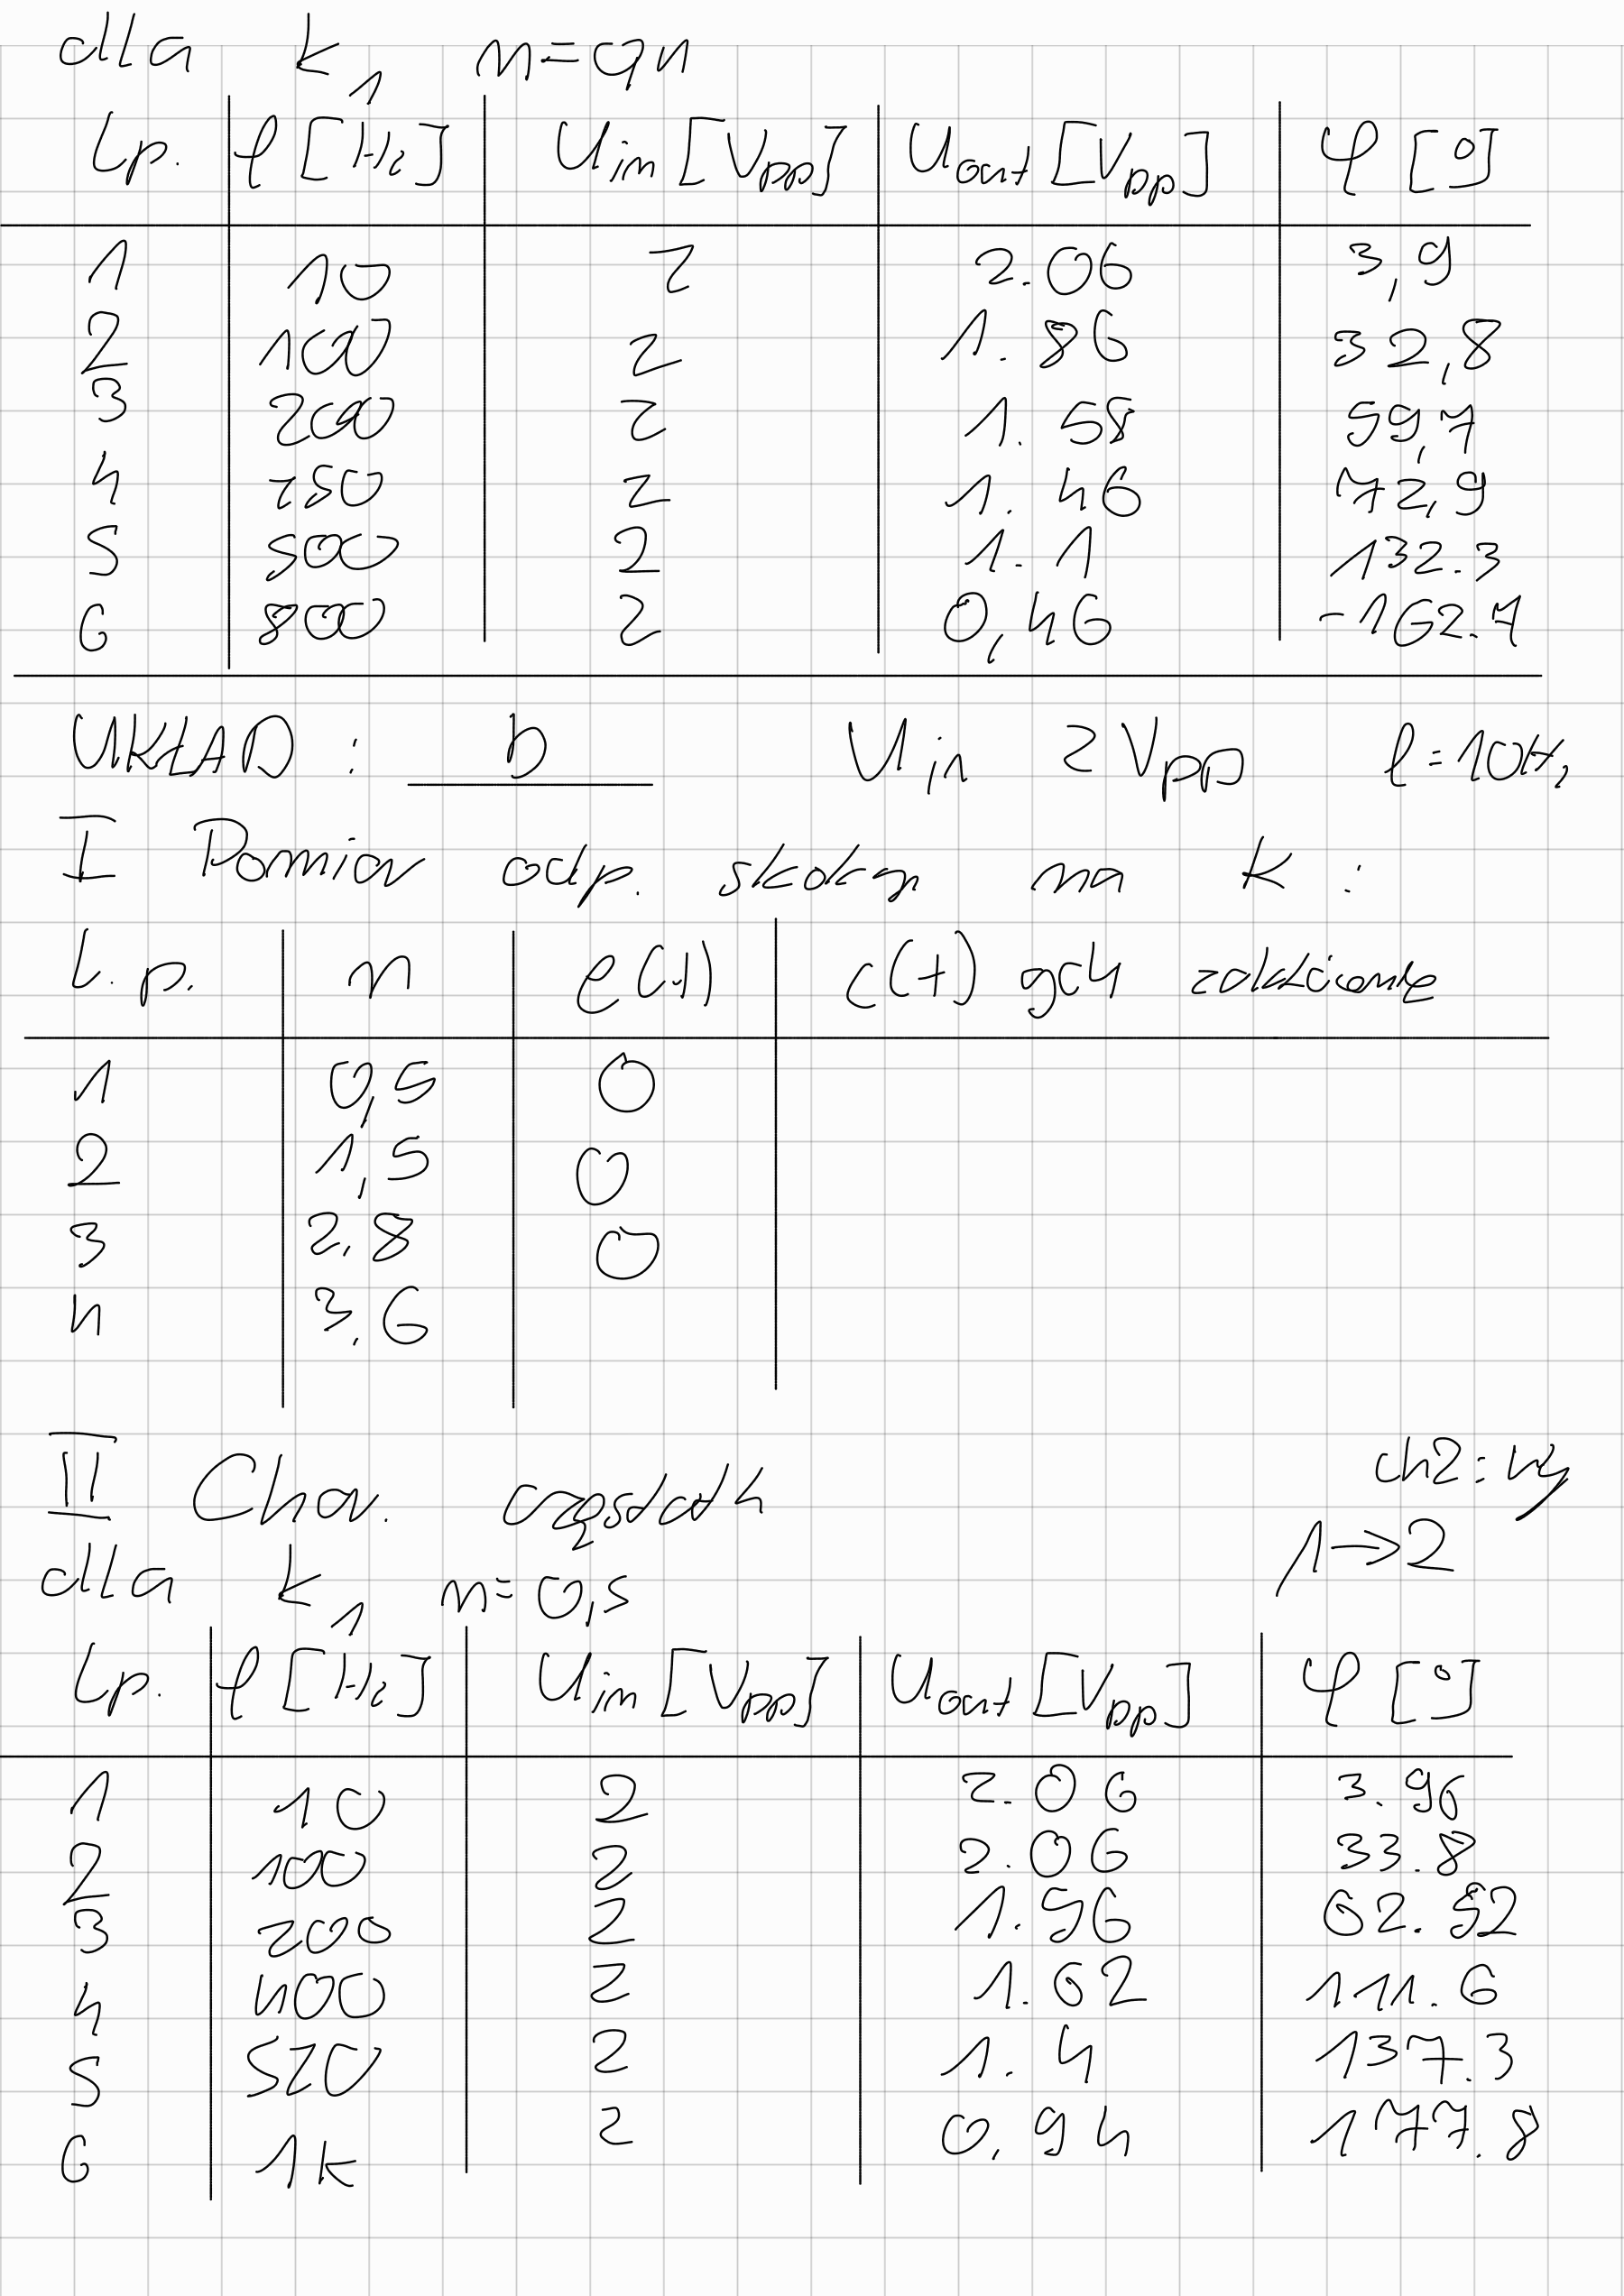
\includegraphics[width=\textwidth]{zdjecia/2.png}
			\caption{Zdjęcie pomiarów 2.}
			\label{fig:pomiar2}
		\end{subfigure}
		\caption{Zdjęcia wykonane podczas laboratorium.}
	\end{figure}
	
	\textbf{W ramach ćwiczenia dokonano identyfikacji następujących obiektów dynamicznych.}
	
	\subsection{Układ inercyjny pierwszego rzędu}
	
	Transmitancja obiektu ma postać:
	\begin{equation}
		G(s) = \frac{k_p}{1 + sT_p}
	\end{equation}
	
	W celu identyfikacji obiektu inercyjnego pierwszego rzędu na jego wejście podano sygnał prostokątny o amplitudzie międzyszczytowej równej \(2\,\text{V}\). Odpowiedź skokowa systemu została zarejestrowana przy użyciu oscyloskopu cyfrowego, a dane pomiarowe zapisano w formacie CSV. Na podstawie zarejestrowanego przebiegu wyznaczono parametry układu za pomocą poniższych zależności.
	
	Wzmocnienie statyczne \(k_p\):
	\begin{equation}
		h(t)\big|_{t \to \infty} = k_p
	\end{equation}
	
	Stała czasowa \(T_p\):
	\begin{equation}
		h(t) = k_p(1-e^{-t/T_p})
	\end{equation}
	Podstawiając czas $t$ równy stałej czasowej $T_p$, otrzymujemy:
	\begin{equation}
		h(T_p) = k_p(1-e^{-T_p/T_p}) = k_p(1-e^{-1})
	\end{equation}
	Wartość $e^{-1}$ jest stałą i wynosi w przybliżeniu $0{,}368$, zatem:
	\begin{equation}
		h(T_p) \approx k_p(1-0{,}368) = 0{,}632 \cdot k_p
	\end{equation}
	Oznacza to, że po czasie równym stałej czasowej $T_p$ odpowiedź obiektu osiąga 63,2\% swojej wartości ustalonej.
	
	\noindent \textbf{Wyznaczone wartości parametrów układu są następujące:}
	\begin{itemize}
		\item $k_p = 0{,}871$ 
		\item $T_p = 0{,}78$ ms
	\end{itemize}
	
	\noindent \textbf{Parametry obliczone z charakterystyk częstotliwościowych:}
	\begin{itemize}
		\item Wzmocnienie $k_p$ obliczono ze wzoru:
	\end{itemize}
	
	\begin{equation}
		M(f)=\frac{A_{wy}}{A_{we}}
	\end{equation}
	
	Z pomiaru przy najniższej częstotliwości (10 Hz) mamy
	\begin{equation}
		k_p \approx M(10\ \text{Hz}) = \frac{1{,}71}{2{,}03} = 0{,}842.
	\end{equation}
	
	Wartość modułu przy częstotliwości granicznej spełnia
	\begin{equation}
		M(\omega_{3\text{dB}})=\frac{k_p}{\sqrt{2}} \approx \frac{0{,}842}{\sqrt{2}} = 0{,}595.
	\end{equation}
	
	Z tabeli widzimy, że częstotliwość wynosi:
	\[
	f_{3\text{dB}} \approx 210\ \text{Hz}.
	\]
	
	Stąd stała czasowa:
	\begin{equation}
		T_p = \frac{1}{\omega_{3\text{dB}}} = \frac{1}{2\pi f_{3\text{dB}}}
		\approx \frac{1}{2\pi\cdot 210} = 0{,}758\ \text{ms}.
	\end{equation}
	
	\noindent \textbf{Parametry wyznaczone za pomocą skryptów MATLABowych:}
	\begin{itemize}
		\item $k_p = 0{,}8366$ 
		\item $T_p = 0{,}74$ ms
	\end{itemize}
	
	\noindent \textbf{Porównanie odpowiedzi skokowych modeli otrzymanych różnymi metodami:}
	Dane wejściowe: \\
	Vin = 2 [Vpp]\\
	f = 10 [Hz]
		
	\begin{figure}[H]
		\centering
		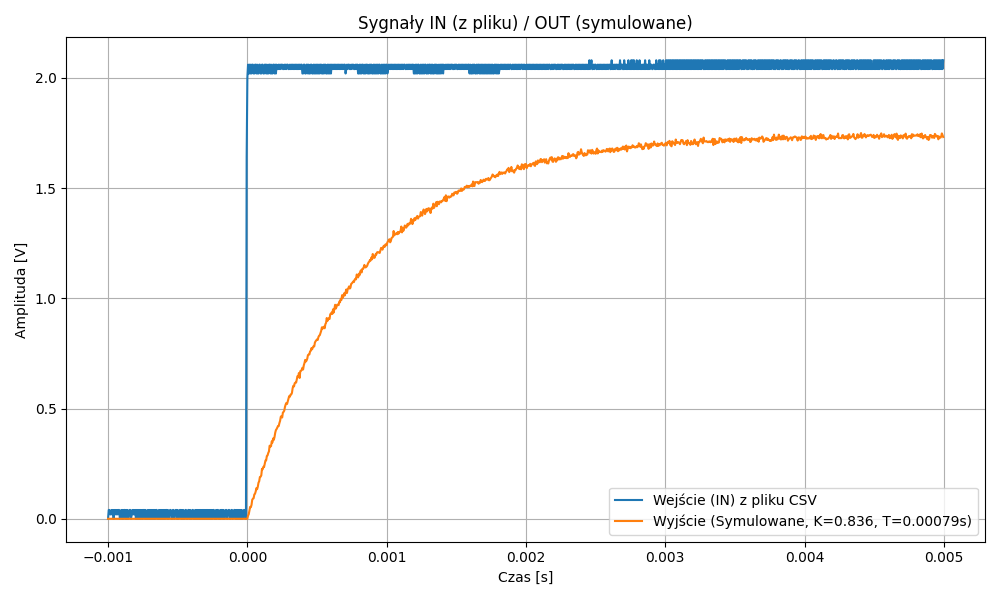
\includegraphics[width=1\linewidth]{zdjecia/OdpSkokowa1.png}
		\caption{Odpowiedzi skokowe układu inercyjnego pierwszego rzędu}
		\label{fig:OdpSkokowa1}
	\end{figure}
	
	\noindent \textbf{Porównanie charakterystyk Bodego otrzymanych różnymi metodami:}
		\begin{figure}[H]
		\centering
		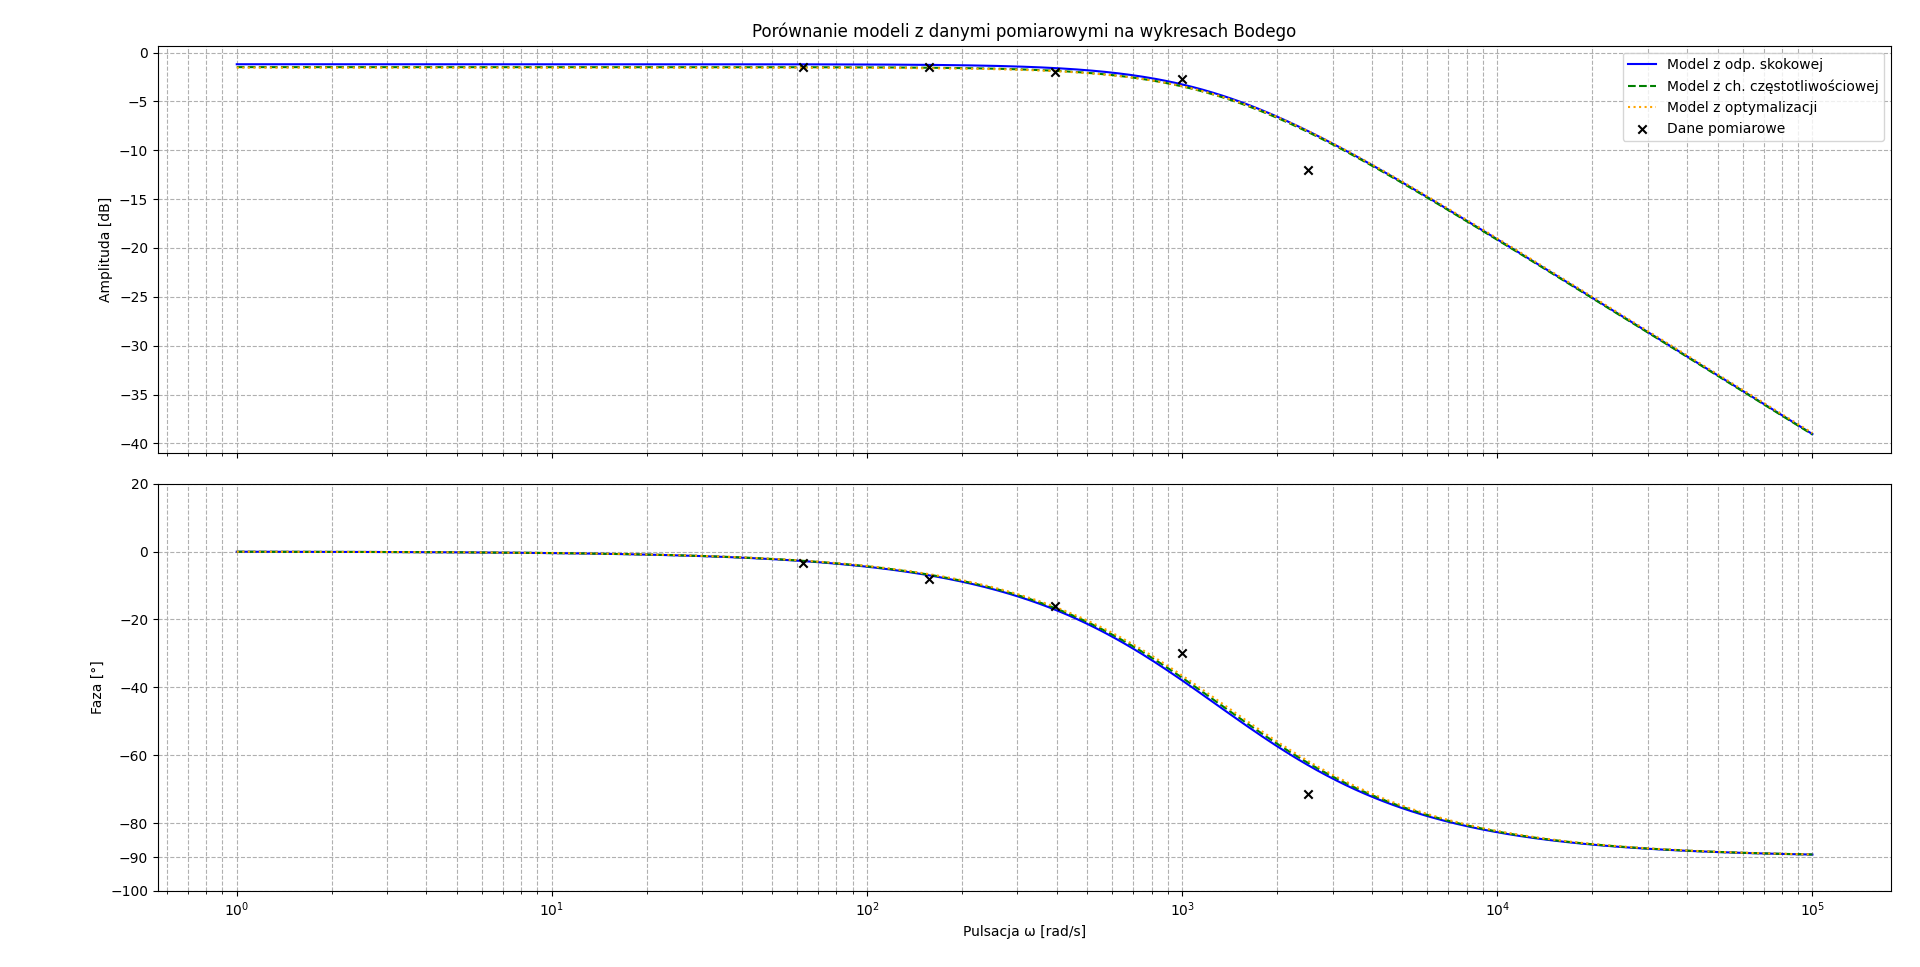
\includegraphics[width=1\linewidth]{zdjecia/Body1.png}
		\caption{Charakterystyki Bodego układu inercyjnego pierwszego rzędu}
		\label{fig:Body1}
	\end{figure}
	
	Porównanie parametrów uzyskanych za pomocą trzech różnych metod identyfikacji wykazało bardzo dużą zgodność, która jest potwierdzona wizualnie na wykresie odpowiedzi skokowych (Rysunek 2). Świadczy to o wiarygodności wykonanych pomiarów oraz poprawności przyjętego modelu matematycznego. Zarejestrowana odpowiedź skokowa, przedstawiona na Rysunku 2, nie wykazuje przeregulowania, co stanowi typową cechę tego typu systemów. Właściwości obiektu jako filtru dolnoprzepustowego przejawiają się w tłumieniu składowych o wysokich częstotliwościach oraz w przesunięciu fazowym, które dla dużych częstotliwości dąży do -90°.
	
	\subsection{Układ inercyjny pierwszego rzędu z opóźnieniem transportowym}
	
	Transmitancja obiektu ma postać:
	\begin{equation}
		G(s) = \frac{k_p}{1 + sT_p} e^{-sT_0}
	\end{equation}
		
	\noindent \textbf{Parametry $k_p$ i $T_p$ przyjęto takie same jak dla układu inercyjnego pierwszego rzędu, 
		ponieważ wprowadzenie opóźnienia transportowego $T_0$ nie wpływa na wzmocnienie ani stałą czasową, a jedynie powoduje dodatkowe przesunięcie fazowe.}
	
	\subsection{Układ całkujący}
	Transmitancja obiektu jest postaci:
	\begin{equation}
		G(s) = \frac{1}{sT_i}
	\end{equation}
	
	\noindent \textbf{Parametry zmierzone na uczelni:}
	\begin{itemize}
		\item $T_i = 0{,}5$ s % <-- Tutaj wstaw swoje zmierzone wartości
	\end{itemize}
	
	\noindent \textbf{Parametry obliczone z charakterystyk częstotliwościowych:}
	\begin{itemize}
		\item Stałą $T_i$ wyznacza się z pulsacji $\omega_0$, dla której charakterystyka amplitudowa przecina oś 0 dB.
		$$|G(j\omega_0)| = \frac{1}{\omega_0 T_i} = 1 \implies T_i = \frac{1}{\omega_0}$$
		Dla przykładowego $\omega_0 = 2$ rad/s, $T_i=0,5$ s.
	\end{itemize}
	
	\noindent \textbf{Parametry wyznaczone za pomocą skryptów MATLABowych:}
	\begin{itemize}
		\item $T_i = 0{,}51$ s % <-- Tutaj wstaw wartości z Matlaba
	\end{itemize}
	
	\subsection{Układ drugiego rzędu}
	Transmitancja obiektu jest postaci:
	\begin{equation}
		G(s) = \frac{k}{1+s 2\zeta T + s^2 T^2}
	\end{equation}
	
	\noindent \textbf{Parametry zmierzone na uczelni:}
	\begin{itemize}
		\item $k = 1{,}0$ % <-- Tutaj wstaw swoje zmierzone wartości
		\item $\zeta = 0{,}4$ % <-- Tutaj wstaw swoje zmierzone wartości
		\item $T = 0{,}1$ s % <-- Tutaj wstaw swoje zmierzone wartości
	\end{itemize}
	
	\noindent \textbf{Parametry obliczone z charakterystyk częstotliwościowych:}
	\begin{itemize}
		\item Parametry wyznacza się z pulsacji rezonansowej $\omega_r$ i wartości szczytu rezonansowego $M_r$.
	\end{itemize}
	
	\noindent \textbf{Parametry wyznaczone za pomocą skryptów MATLABowych:}
	\begin{itemize}
		\item $k = 1{,}02$ % <-- Tutaj wstaw wartości z Matlaba
		\item $\zeta = 0{,}42$ % <-- Tutaj wstaw wartości z Matlaba
		\item $T = 0{,}09$ s % <-- Tutaj wstaw wartości z Matlaba
	\end{itemize}
	
	\subsection{Układ nieminimalnofazowy}
	Transmitancja przykładowego obiektu nieminimalnofazowego:
	\begin{equation}
		G(s) = k \frac{1-sT_z}{1+sT_p}
	\end{equation}
	
	\noindent \textbf{Parametry zmierzone na uczelni:}
	\begin{itemize}
		\item $k = 1{,}0$ % <-- Tutaj wstaw swoje zmierzone wartości
		\item $T_z = 0{,}05$ s % <-- Tutaj wstaw swoje zmierzone wartości
		\item $T_p = 0{,}1$ s % <-- Tutaj wstaw swoje zmierzone wartości
	\end{itemize}
	
	\noindent \textbf{Parametry obliczone z charakterystyk częstotliwościowych:}
	\begin{itemize}
		\item Obecność zera w prawej półpłaszczyźnie objawia się dodatkowym, narastającym opóźnieniem fazowym.
	\end{itemize}
	
	\noindent \textbf{Parametry wyznaczone za pomocą skryptów MATLABowych:}
	\begin{itemize}
		\item $k = 1{,}0$ % <-- Tutaj wstaw wartości z Matlaba
		\item $T_z = 0{,}051$ s % <-- Tutaj wstaw wartości z Matlaba
		\item $T_p = 0{,}102$ s % <-- Tutaj wstaw wartości z Matlaba
	\end{itemize}
	
	% =====================================
	%          PODSUMOWANIE
	% =====================================
	\section{Wnioski}
	% Wnioski do uzupełnienia po przeprowadzeniu pełnej analizy
	Ćwiczenie pozwoliło na praktyczne zapoznanie się z metodami identyfikacji obiektów dynamicznych. Wyznaczono parametry modeli matematycznych na podstawie trzech różnych metod: pomiarów bezpośrednich, analizy charakterystyk częstotliwościowych oraz dopasowania z użyciem narzędzi numerycznych. Porównanie wyników pozwoli na ocenę dokładności i przydatności każdej z metod.
	
\end{document}